\section{Automatic Differentiation}
In the following, we will consider a \say{set} of data points
\begin{equation*}
    X\in\R^{N\times d}
\end{equation*}
made of $N$ inputs of size $d$, and targets
\begin{equation*}
    Y\in\Y^n
\end{equation*}
where $\Y$ is an arbitrary set. It can be for instance $\Y=\R$ is the case of regression, a finite set such as $\iset{1}{C}$ in the case of classification, or $\Y=\R^{d'}$ in a more general setup.

\subsection{Introduction}
As stated previously, neural networks is a very expressive class of functions. However, the associated optimization problem is in general non-convex, giving very few theoretical guarantees and no closed-form expression. In practice, this is not an issue, since such optimization problem can be solved using \emph{gradient descent}.
\subsubsection{Loss function}

Gradient descent is done by minimizing the average of a differentiable loss function $\L:\Y\times\Y\to\R$. For instance, for regression, we might choose the squared error:
\begin{equation*}
    \L(\hat{y}, y) = (\hat{y}-y)^2
\end{equation*}
For classification, we might choose the logistic loss. Its expression for a two-classes model (that is $y\in\{0, 1\}$) is:
\begin{equation*}
    \L(\hat{y}, y) = y\log\hat{y} + (1-y)\log(1-\hat{y})
\end{equation*}
More generally, for a $C$-classes model (that is $y\in\iset{1}{C}$), the cross-entropy loss is:
\begin{equation*}
    \L(\hat{y}, y) =  \sum_{c=1}^C y_c \log \hat{y}_c
\end{equation*}
The average of the loss function is then given by:
\begin{equation*}
    J(f) = \frac{1}{N}\sum_{n=1}^N \L\left(f(X_n), Y_n\right)
\end{equation*}
which we will try to minimize.

\subsubsection{Gradient descent}
The idea behind gradient descent is therefore to be able to compute the gradient of $\L$ with respect to the paramters $\theta$ for each point of the dataset:
\begin{figure}[H]
    \centering 
    \begin{minipage}{0.4\textwidth}
    \begin{minted}[escapeinside=||, mathescape=true]{python}
for epoch in range(EPOCHS):
    for x, y in zip(X, Y):
        compute |$\nabla_\theta\L$|
        |$\theta = \theta - \gamma\nabla_\theta\L$|
    \end{minted}
    \end{minipage}
    \caption{Pseudo-code of gradient descent}
\end{figure}
The only remaining challenge is the computation of $\nabla_\theta\L$, preferably automatically; this is the problem which we will address in this chapter.

\subsection{Optimization methods}
\subsubsection{Stochastic Gradient Descent}
\subsubsection{Batch gradient descent}
\subsubsection{Minibatch gradient descent}
\subsubsection{Newton's method}

\subsection{Computing gradients}
\subsubsection{By hand}
The most straightforward approach to computing $\nabla_\theta\L$ would be to derive it on paper. Nevertheless, this is complicated, as it involves very long computations using matrix calculus.

Furthermore, this approach is not modular, as changing the loss function or adding a layer requires to re-derive the gradient from scratch. Such a method does not scale: if the computations can be done in a reasonable amount of time for small models using linear and activation layers, complex models introduced in the next chapters have enormous gradient expressions, making the computation way too long and tidious to be done by hand.

\subsubsection{Numerical differentiation}
\subsubsection{Symbolic differentiation}

\subsection{Automatic differentiation}
\subsubsection{Computational Graphs}
Automatic differentiation uses a data structure called \emph{Computational Graphs} to represent the computation that is happening inside the model.
\begin{figure}[H]
    \centering
    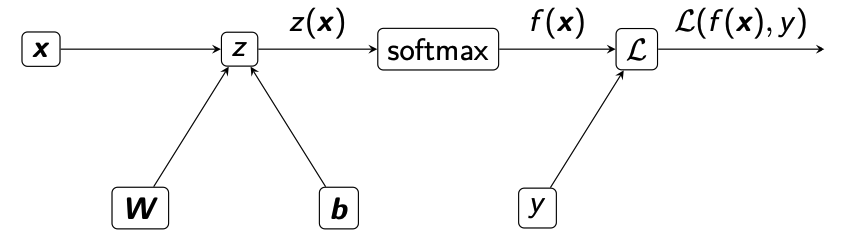
\includegraphics[width=.7\textwidth]{images/computational-graph.png}
    \caption{Computational graph for $\L(\softmax(Wx+b), y)$}
    \label{fig:computational-graph}
\end{figure}
In Figure \ref{fig:computational-graph}, reading from left to right, we can see that the weights $W$, the biases $b$ and the input $x$ are combined to create a function $z(x)$; to the result of this operation is applied $\softmax$, creating $f(x)$. Finally, $f(x)$ is combined with $y$ using the loss function $\L$, giving the final result of the computation, $\L(f(x), y)$.

Computational graphs can then be used to apply the main algorithm to compute the gradient, called \emph{backpropagation}. We will illustrate its behavior by considering the function $f(x, y, z) = (x+y)\times z$, to which is associated the following computational graph:
\begin{figure}[H]
    \centering
    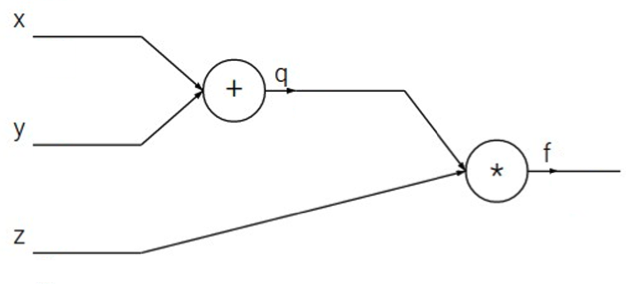
\includegraphics[width=.5\textwidth]{images/simple-graph.png}
    \caption{Computational graph for $f(x, y, z) = (x+y)\times z$}
\end{figure}

\subsubsection{Forward pass}
The first step of backpropagation is to compute the outputs during a \emph{forward pass}. This is simply done by replacing each input by its numerical value, and applying the operations described by the nodes of the graph. Using $x=-2$, $y=5$, $z=-4$ in the previous example yields:
\begin{figure}[H]
    \centering
    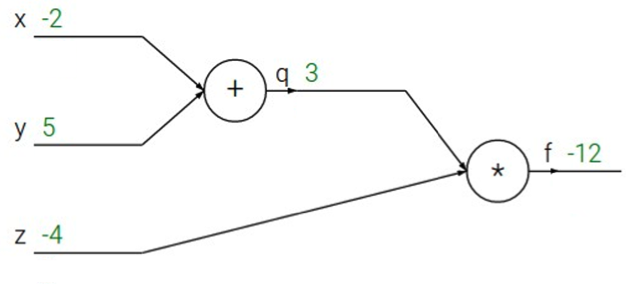
\includegraphics[width=.5\textwidth]{images/forward-graph.png}
    \caption{Forward pass}
\end{figure}

\subsubsection{Backward pass}
The backward pass allows us to compute the derivatives, in our case $\partfrac{f}{x}$, $\partfrac{f}{y}$ and $\partfrac{f}{z}$. Instead of computing the value at each node from left to right (forward pass), we will compute the values of the derivatives from right to left, starting from the output (backward pass).

\begin{itemize}
    \item Starting from the output node, we have that $\partfrac{f}{f}=1$.
    \item Going backward to the $z$ input node, we have that $\partfrac{f}{z}=q$, since $f=qz$. We can then use the results of the forward pass to find the value of $q$, and deduce $\partfrac{f}{z}=3$.
    \item Similarly, $\partfrac{f}{q}=z=-4$.
    \item Going further back into the graph, we aim at computing $\partfrac{f}{y}$. Using chain rule, we know that:
    \begin{equation*}
        \partfrac{f}{y}=\partfrac{q}{y}\partfrac{f}{q}
    \end{equation*}
    This equation can be interpreted in terms of \say{gradient stream}: we want to compute the \emph{downstream gradient} $\partfrac{f}{y}$, that is the gradient \say{after the node}. This gradient can therefore be expressed using the chain rule as the product of the \emph{local gradient} $\partfrac{q}{y}$ and the \emph{upstream gradient} $\partfrac{f}{q}$, that is the gradient computed at the previous node.
    \begin{equation*}
        \underbrace{\partfrac{f}{y}}_{\textnormal{Downstream}}=\underbrace{\partfrac{q}{y}}_{\textnormal{Local}} \underbrace{\partfrac{f}{q}}_{\textnormal{Upstream}}
    \end{equation*}
    Like in previous cases, we can compute the local gradient $\partfrac{q}{y}=1$ since $q=x+y$. The upstream gradient is also known at this point of the pass, due to the backward direction, hence $\partfrac{f}{y}=1\times-4=-4$
    \item The same approach using the chain rule can be used for $\partfrac{f}{x}=\partfrac{q}{x}\partfrac{f}{q}=1\times -4=-4$.
\end{itemize}

\subsubsection{Modularity}
A benefit of backpropagation is its modularity: the gradient computation can be broke down into the computation of the downstream gradient knowing the upstream gradient and the local gradient of the node. 

Consider for instance a function $f$ taking $x$ and $y$ as inputs, and producing an output $z$. This function is a node somewhere in a possibly very complex computational graph, but we do not need the whole information about the rest of the computation: to compute the downstream gradient, we only need local information, that is upstream and local gradients. 

We are given the upstream gradient of the loss that we want to compute with respect to our output, $\partfrac{\L}{z}$. Our goal is now simply to propagate the gradient computation by providing the downstream derivatives, that is $\partfrac{\L}{x}$ and $\partfrac{\L}{y}$. Since we know the expression of $f$, we are able to compute the local derivatives $\partfrac{z}{x}$ and $\partfrac{z}{y}$; using chain rule, we can therefore provide the downstream gradient.
\begin{figure}[H]
    \centering
    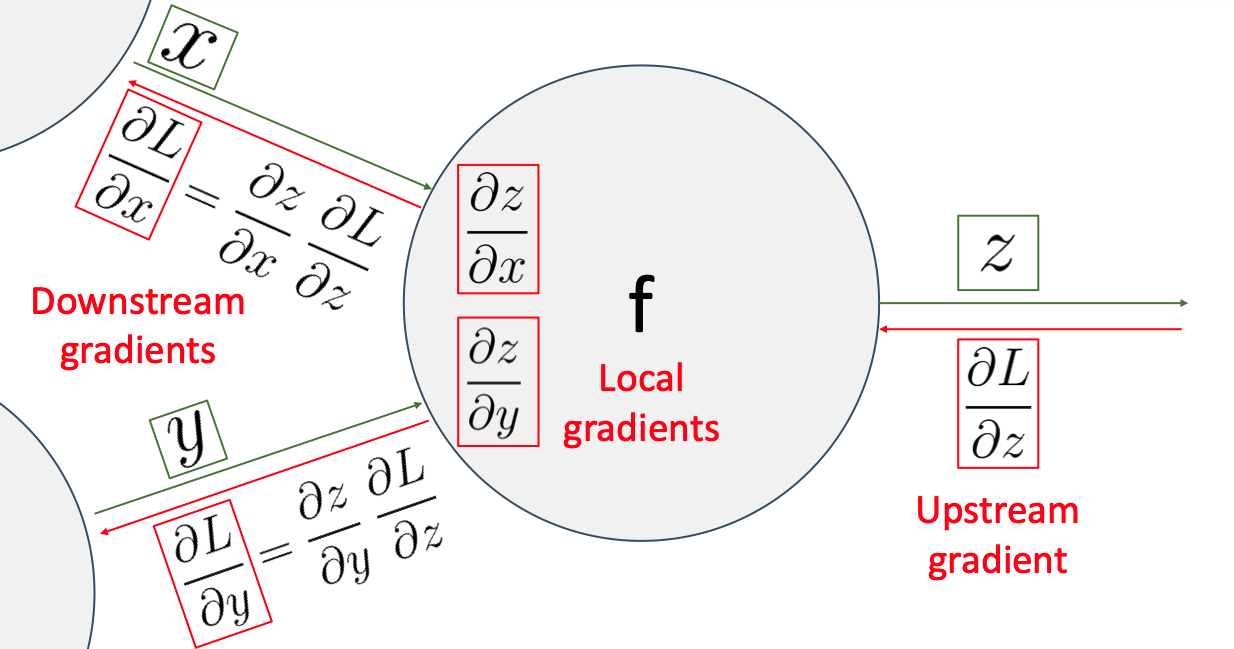
\includegraphics[width=.6\textwidth]{images/modularity.png}
    \caption{Local process of computing the downstream gradient}
\end{figure}